\section{Methoden und Daten}

In dieser Untersuchung wird ein Datensatz verwendet, der im Rahmen der Publikation "Progress of Nutrition Vol. 23 No. 2 (2021)" veröffentlicht und in der Studie "Classification of Pistachio Species Using Improved k-NN Classifier"\cite{Ozkan.2021} vorgestellt wurde. Der Datensatz ist öffentlich zugänglich und speziell für die Klassifikation zweier Pistazienarten (\glqq{}Kirmizi\grqq{} und \glqq{}Siirt\grqq{}) erstellt worden. Für diese Studie wurden 2148 hochauflösende Bilder von diesen zwei Pistazienarten aufgenommen. Anhand dieser Aufnahmen konnten die Merkmale gemessen werden.

\section*{Explorative Datenanalyse} 
Der Datensatz beinhaltet zwei Versionen mit einem unterschiedlichen Umfang an Merkmalen: eine Version umfasst 16 Features, während die andere Version 28 Features bietet. Für die Zwecke dieses Projekts wird die Version mit 16 Features verwendet. Die Auswahl dieser Version erfolgte aufgrund der Tatsache, dass die zusätzlichen 12 Features Farbmerkmale der Pistazien darstellen, welche in dieser spezifischen Untersuchung nicht berücksichtigt werden.

Die für dieses Projekt verwendeten Merkmale lassen sich in die folgenden Kategorien unterteilen:

\subsection*{Morphologische Merkmale (12 Features):}
\begin{itemize}
	\item Fläche (Area)
	\item Umfang (Perimeter)
	\item Hauptachse (Major\_Axis)
	\item Nebenachse (Minor\_Axis)
	\item Exzentrizität (Eccentricity)
	\item Äquivalentdurchmesser (Eqdiasq)
	\item Solidität (Solidity)
	\item Konvexe Fläche (Convex\_Area)
	\item Ausdehnung (Extent)
	\item Seitenverhältnis (Aspect\_Ratio)
	\item Rundheit (Roundness)
	\item Kompaktheit (Compactness)
\end{itemize}

\subsection*{Formmerkmale (4 Features):}
\begin{itemize}
	\item Formfaktor 1 (Shapefactor\_1)
	\item Formfaktor 2 (Shapefactor\_2)
	\item Formfaktor 3 (Shapefactor\_3)
	\item Formfaktor 4 (Shapefactor\_4)
\end{itemize}

Die vier Formmerkmale sind weitere mathematische Zusammenfassungen zwischen einzelnen morphologischen Merkmalen.
Was sich genau hinter den Bezeichnungen versteckt lässt sich unter \parencite[4]{Ozkan.2021} in Tabelle 1 nachlesen.

Eine genauere Betrachtung könnte helfen um Abhängigkeiten zwischen den Merkmalen zu erkennen und später Merkmale nicht zu vergleichen, die nicht direkt Abhängig zu einander sind.

- kurze explorative Datenanalyse mit Visualisierung des Datensatzes
- Aufbereitung der Daten (ggf. Skalierung, Entfernung von fehlerhaften Daten etc.)
- Aufteilung der Daten in Trainings- und Testdaten
- Pro Klassifikationsmethode ist je mindestens einen Parameter variieren
	Wahl des jeweiligen Parameters begründen
	Einfluss des Parameters auf die Performanz der Methode visualisieren
	Gute Parametereinstellungen begründet wählen
	


\section{Ergebnisse}

- Bewertung mit der Klassifikationsleistung mit geeigneten Qualitätsmaßen (z.B. Genauigkeit, Recall, Precision oder Sensitivität \& Spezifität)
- Visualisierung der Ergebnisse

\begin{figure}
	\centering
	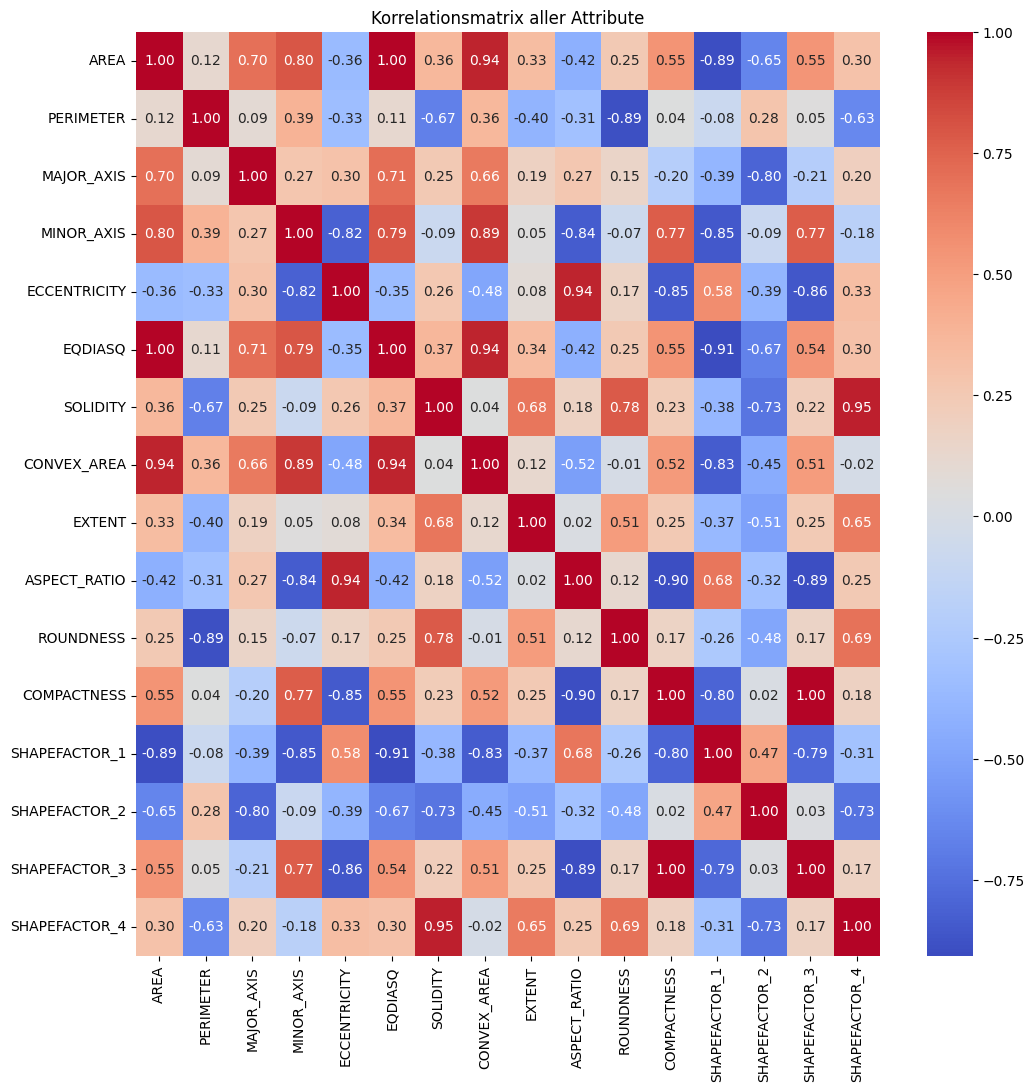
\includegraphics[width=\columnwidth]{images/korrelationsmatrix_aller_attribute}
	\caption{}
	\label{fig:korrelationsmatrixallerattribute}
\end{figure}
